%=============================================================================
% Thesis Template in LaTex
%
% File:  Varianten -- Fallstudie
% Author(s): Jürgen Hackl <hackl@ibi.baug.ethz.ch>
%            Clemens Kielhauser <kielhauser@ibi.baug.ethz.ch>
%
% Creation:  27 Jan 2014
% Time-stamp: <Tue 2013-08-13 20:14 juergen>
%
% Copyright (c) 2014 Infrastructure Management Group (IMG)
%               http://ibi.ethz.ch
%
% More information on LaTeX: http://www.latex-project.org/
%=============================================================================

% Unterkapitel Varianten
% ---------

Die folgenden Varianten habe ich, im Rahmen der Optimierung der Verkehrssituation am Bahnübergang Brunnenstrasse erarbeitet, um die Situation für die nächsten vierzig Jahre nachhaltig zu verbessern. Anschliessend an die Darstellung der Varianten folgt eine Übersicht der wichtigsten Eigenschaften und Parameter der Infrastrukturen, die für die Berechnung der Kosten verwendet werden. \\
Die Gesamtlänge des betrachteten Infrastrukturabschnitt beträgt für alles Variante 80 Meter.


\subsection{Variante \ 1}
\label{subsec:V1}
	
Die Variante 1 stellt den Ist-Zustand der Infrastruktur dar. In dieser Variante beträgt die durchschnittliche Wartezeit pro Nutzer, wie in Abschnitt \ref{sub:Reisezeit} erläutert, 5 Minuten.  Mit dieser Variante kann der jetztige Zustand der Infrastruktur über den betrachteten Zeitraum von vierzig Jahren untersucht werden und so die Option "keine Veränderung Durchführen" überprüft werden. 

%\begin{figure}[h!]
  %\centering
  %\subfloat[][]{\label{img:V1Ü}\includegraphics[width=.6\textwidth]{./figures/1}}
  %\hfill
 % \subfloat[][]{\label{img:V1Q}\includegraphics[width=.4\textwidth]{./figures/1_2}}
%\caption[Variante 1]{Übersicht und Querschnitt der Variante 1}
 % \label{fig:V1}
%\end{figure}

\begin{figure}[h!]
	\centering
	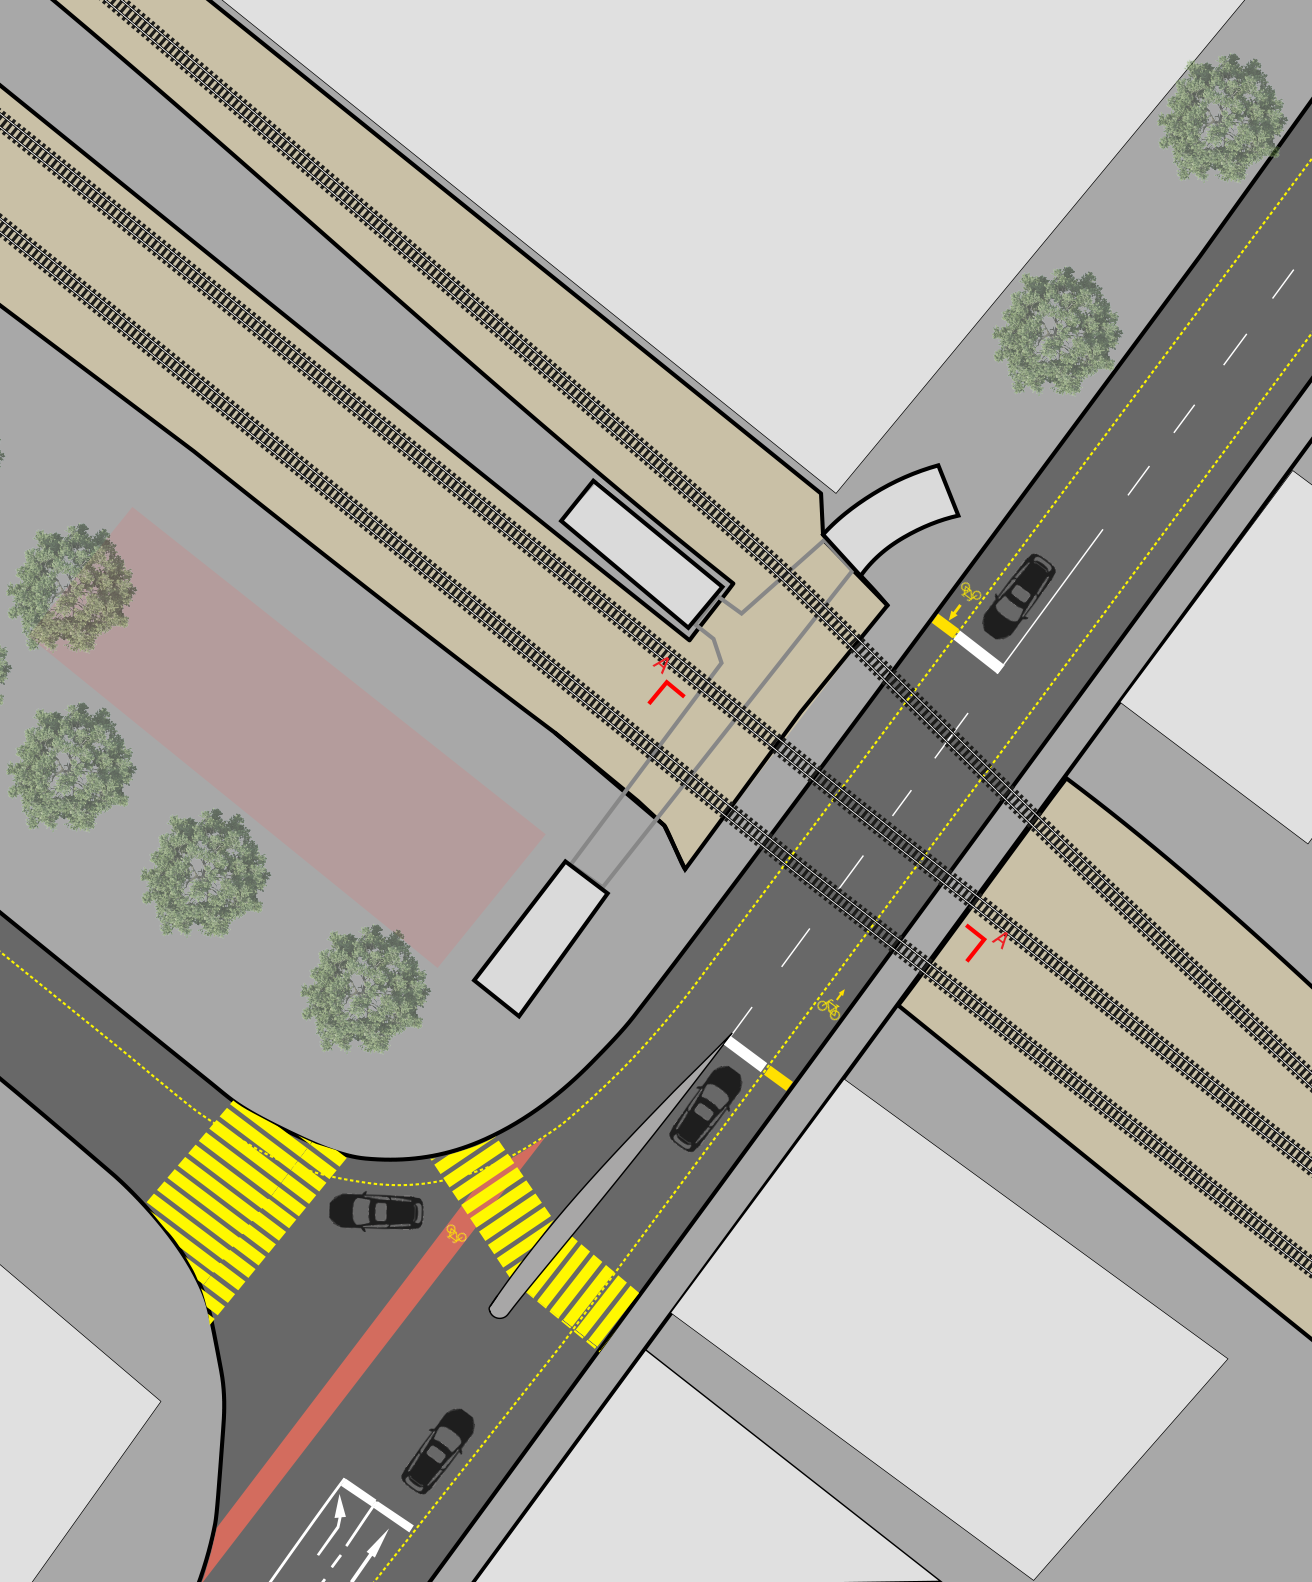
\includegraphics[width=0.65\textwidth]{figures/f-04-05-01-a-V1}
	\caption[Übersicht Variante 1]{Übersicht über die Variante 1}
	\label{img:V1Ü}
\end{figure}

\pagebreak

Um die Verkehrssicherheit der Langsamverkehrsteilnehmer minimal zu erhöhen, ist die Anbringung zweier Velostreifen à je 1.5 Meter Breite geplant. Die angenommene Kapazität der beiden Velostreifen zusammen beträgt 3350 Velo pro Stunde. \\
Die Anbringung der Velostreifen erfordert eine geringfügige verjüngung der Fahrbahn von 4 auf 3.5 Meter pro Fahrbahn. Trotz Verjüngung wird angenommen, dass der zweispurige Strassenabschnitt (eine pro Richtung) eine Kapazität von 2'500 Fahrzeugen pro Stunde aufweist, bei einer geplanten, zulässigen Höchstgeschwindigkeit 50 $km/h$. Unter Berücksichtigung der Situatuion vor Ort wird angenommen, dass die durchschnittlich gefahrenen Geschwindigkeit des MIV 37 $km/h$ beträgt un die der Velofahrer durchschnittlich 15 $km/h$. (\cite{Nacto2018}) (\cite{Mikrozensus2015})

\begin{figure}[h!]
	\centering
	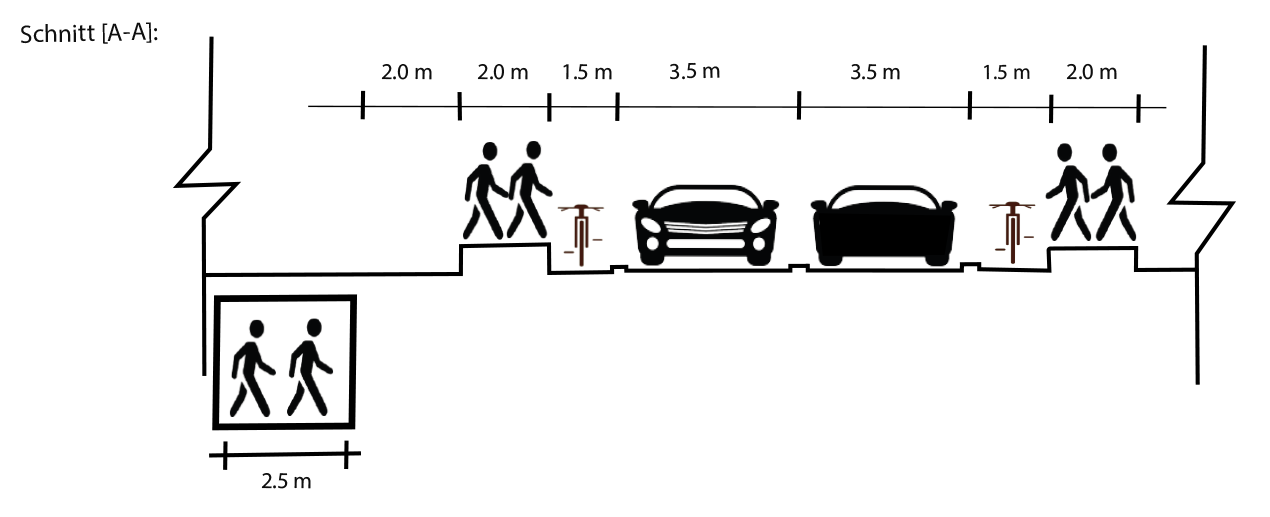
\includegraphics[width=0.7\textwidth]{figures/f-04-05-01-b-V1}
	\caption[Querschnitt Variante 1]{Querschnitt im Schnitt A-A der Variante 1}
	\label{img:V1Q}
\end{figure}

Die Erstellung zweier neuer Radstreifen à je 1.5 Meter Breite kostet gemäss Abschnitt \ref{sub:Unterhalt} 850 CHF pro Laufmeter. Bei einer Gesamtlänge von 80 Meter ergibt sich für den Bau der Variante 1 Kosten im Bereich von 68'000 CHF. (\cite{Baukosten2010}) 

\pagebreak

\subsection{Variante: \ 2}
\label{subsec:V2}
	
Die zweite Variante beinhaltet, wie in Abbildung \ref{img:V2Ü} ersichtlich, den Bau von zwei Velounterführungen, um die lange Wartezeit am Bahnübergang aufgrund der Schliesszeit der Bahnschranken zu verkürzen. Der Zeitverlust der Velofahrer setzt sich demnach in dieser Variante, nur aus dem Zeitverlust der gemäss Abschnitt \ref{sub:Reisezeit} aufgrund des Befahren der Infrastruktur entsteht zusammen. Die für den MIV angesetzte durschnittliche Wartezeit beträgt weiterhin 5'. 

Infolge der Rückklassierung der Brunnenstrasse wird ein Tempo 30 Regime eingeführt. Die angenommene durchschnittlich gefahrene Geschwindgkeit des MIV beträgt somit 30 $km/h$ und für die Velofahrer wird angenommen, dass sie mit durchschnittlich 20 $km/h$ durch die Unterführung fahren können. (\cite{Mikrozensus2015})

%\begin{figure}[h!]
 % \centering
 % \subfloat[][]{\label{img:V2Ü}\includegraphics[width=.6\textwidth]{./figures/2}}
  %\hfill
 % \subfloat[][]{\label{img:V2Q}\includegraphics[width=.4\textwidth]{./figures/2_2}}
%\caption[Variante 2]{Übersicht und Querschnitt der Variante 2}
  %\label{fig:V2}
%\end{figure}

\begin{figure}[h!]
	\centering
	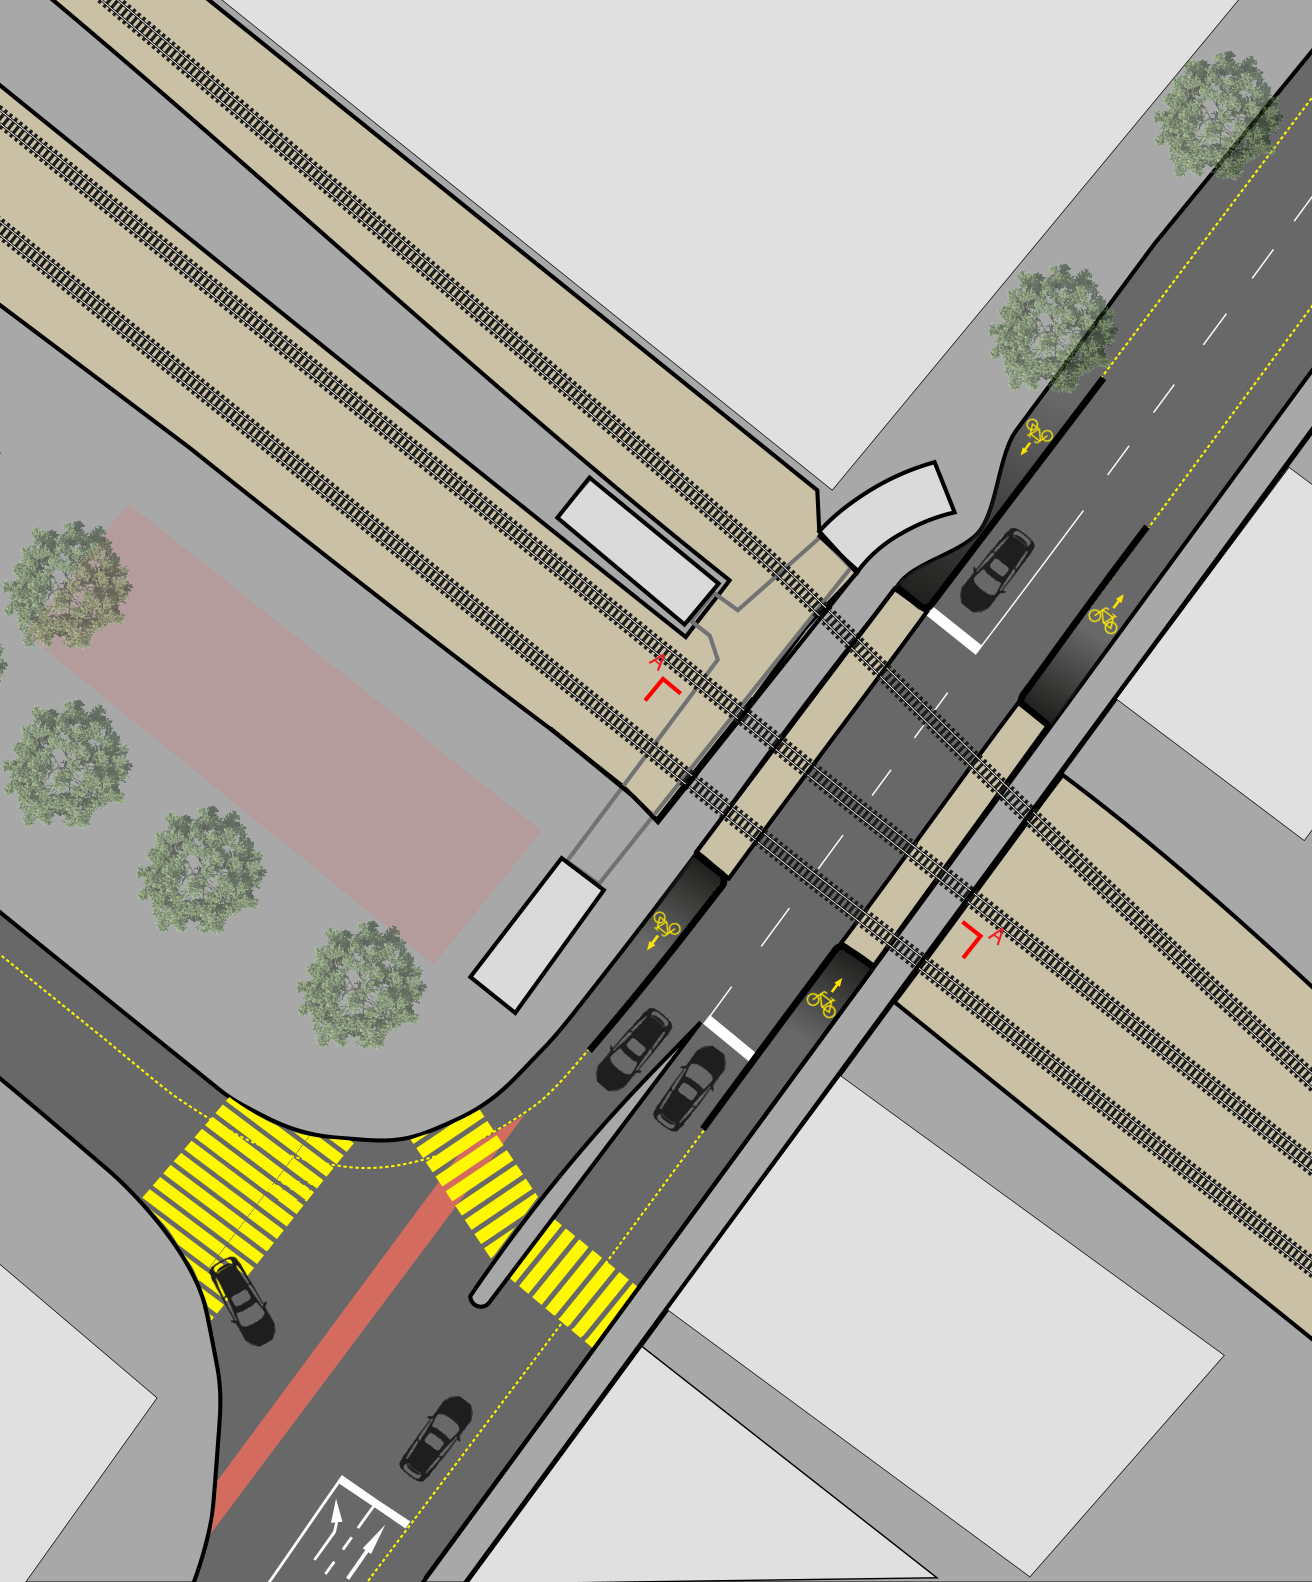
\includegraphics[width=0.65\textwidth]{figures/f-04-05-02-a-V2}
	\caption[Übersicht Variante 2]{Übersicht über die Variante 2}
	\label{img:V2Ü}
\end{figure}

Durch den Bau der beidseitig mit einer lichten breite von 1.5 Meter ausgeführten Velounterführungen, wird einerseits die Verkehrssicherheit der Velofahrer verbessert und andererseits die Kapazität der gesamten Veloinfrastruktur auf 3767 Velos pro Stunde erhöht. Die Gesamtlänge einer Unterführung beträgt in dieser Variante 55 Meter. 

Um diese Unterführung bauen zu können, ist eine weitere verjüngung der Fahrbahn auf 3 Meter erforderlich, was jedoch zu keiner Reduktion der Kapazität des MIV führen wird.  (\cite{Nacto2018})

\begin{figure}[h!]
	\centering
	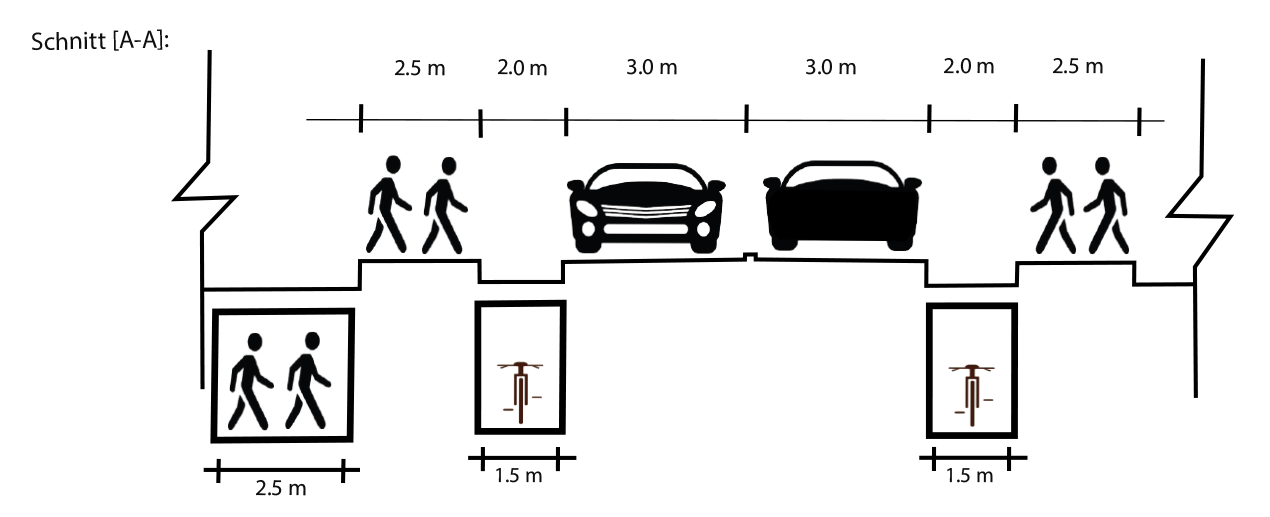
\includegraphics[width=0.7\textwidth]{figures/f-04-05-02-b-V2}
	\caption[Querschnitt Variante 2]{Querschnitt im Schnitt A-A der Variante 2}
	\label{img:V2Q}
\end{figure}

Die prognostizierten Baukosten der Variante 2 werden mithilfe der in Abschnitt \ref{sub:Unterhalt} erläuterten Einheitskosten für den Bau einer Velounterführung und den vorgängig erwähnten Abmessungen der Unterführungen berechnet. Die zu erwartenden Baukosten belaufen sich auf 1.16 Mio. CHF, wobei 520'000 CHF für die vier Rampen und 640'000 CHF für den Bau der Unterführungen unter dem Lastfall Eisenbahn sowie das Anbringen der Velostreifen anfallen. (\cite{Baukosten2010}) 

\pagebreak

\subsection{Variante: \ 3}
\label{subsec:V3}

Die dritte Variante habe ich ausgehend von der Variante 2 entwickelt und ist ein Versuch die Verkehrssicherheit sowie den Fahrkomfort für die Velofahrer zu steigern. Um dies zuerreichen wird, wie in Abbildung \ref{img:V3Ü} ersichtlich ist, die Velounteführung zweispurig ausgeführt, was zur Folge hat, dass die Strasse einspurig über den Bahnübergang geführt werden muss. Diese Strassenführung erfordert die Einführung eines Ampelsystems, was die durchschnittliche Wartezeit für den MIV, bei einem Rotlichtzyklus von einer Minute, auf 7 Minuten erhöht. Für das Ampelsystem wäre eine Busbevorzugungsanalge zu prüfen. \\

Die maximale Höchstgeschwindigkeit beträgt wie in Variante 2 30 $km/h$, wobei angenommen wird, dass die Velofahrer mit durchschnittlich 25 $km/h$ durch die Unterführung fahren können. (\cite{Mikrozensus2015})

%\begin{figure}[h!]
 % \centering
  %\subfloat[][]{\label{img:V3Ü}\includegraphics[width=.6\textwidth]{./figures/3}}
  %\hfill
 % \subfloat[][]{\label{img:V3Q}\includegraphics[width=.4\textwidth]{./figures/3_2}}
%\caption[Variante 3]{Übersicht und Querschnitt der Variante 3}
 % \label{fig:V3}
%\end{figure}

\begin{figure}[h!]
	\centering
	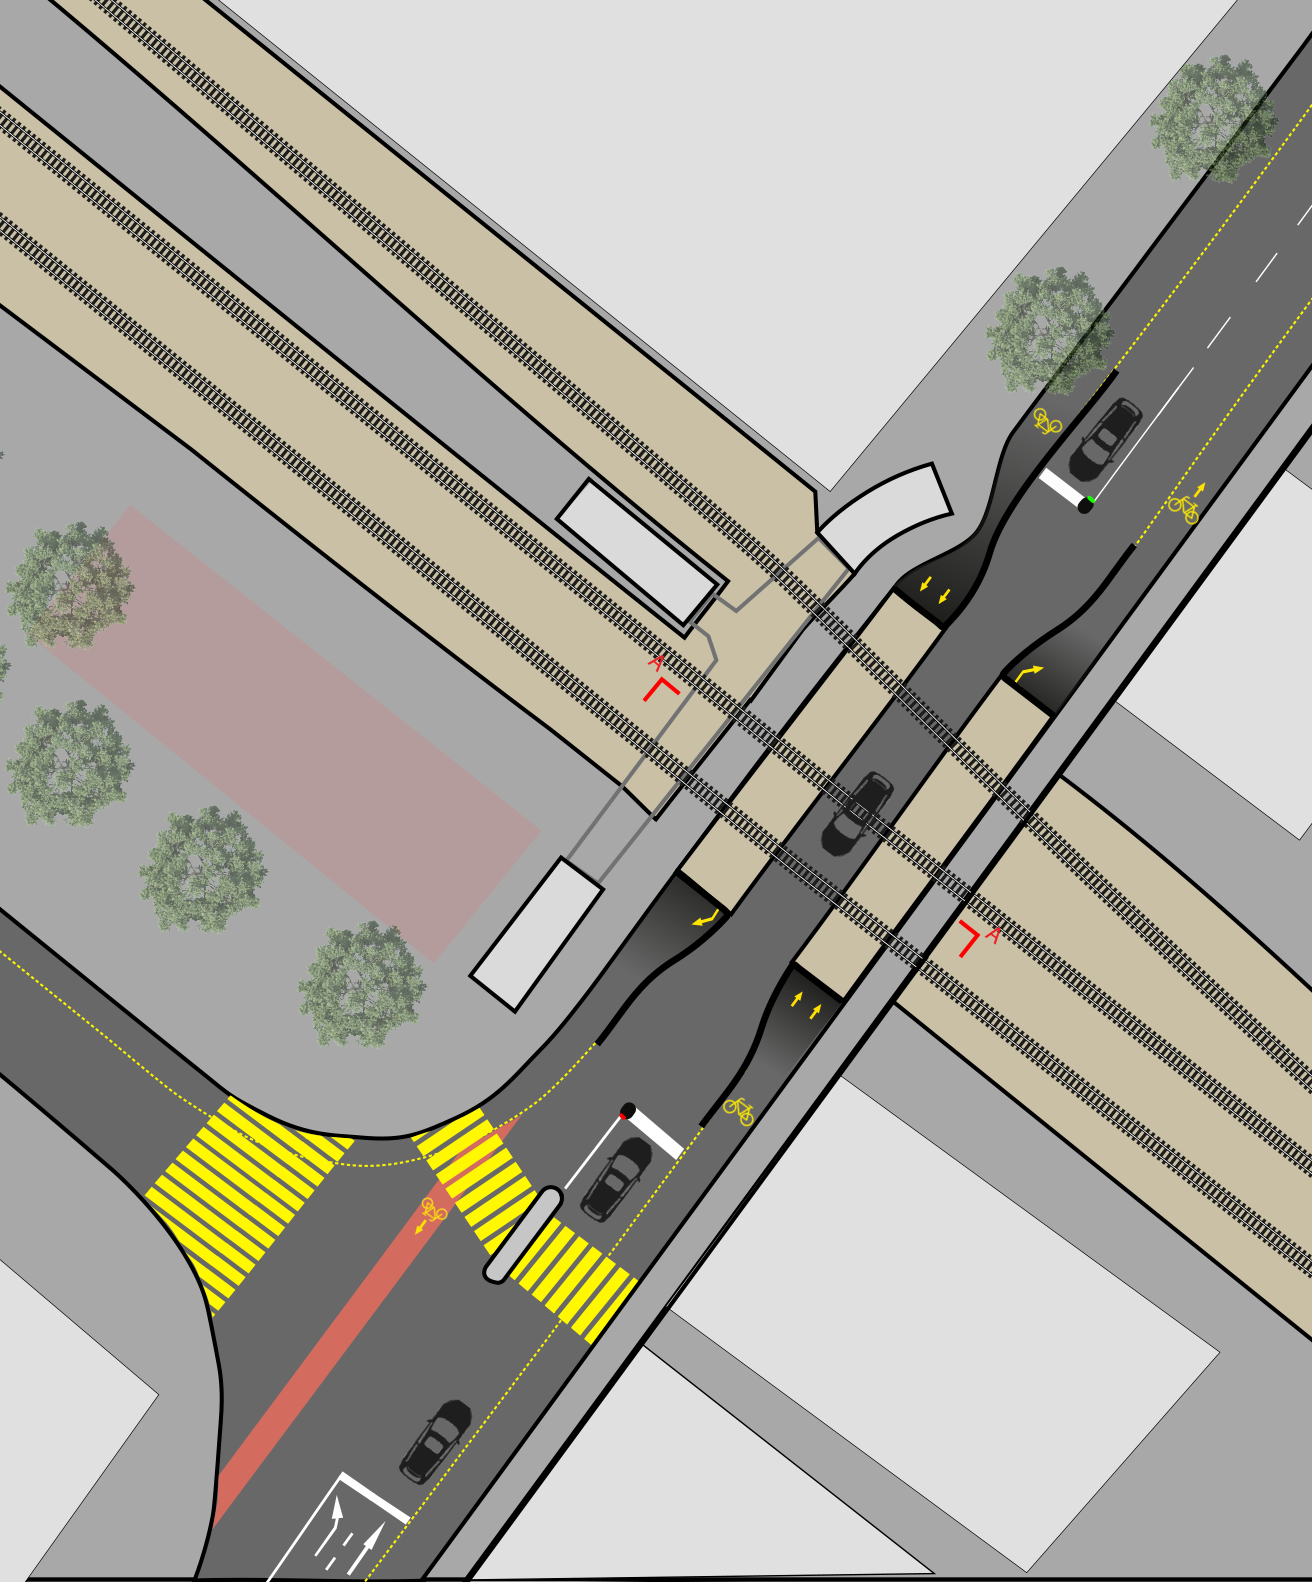
\includegraphics[width=0.65\textwidth]{figures/f-04-05-03-a-V3}
	\caption[Übersicht Variante 3]{Übersicht über die Variante 3}
	\label{img:V3Ü}
\end{figure}

Die lichte Breite der Velounterführung beträgt 2 Meter und die Gesamtlänge einer Unterführung beläuft sich auf 65 Meter. Die zweispurige Strassenführung wird mit Fahrbahnmarkierungen verdeutlicht. Es wird angenommen, dass durch diese Ausführung die Kapazität der gesamten Veloinfrasturktur auf 4600 Velos pro Stunde erhöht wird. (\cite{Nacto2018})

Infolge der Reduktion der Strasseninfrastruktur um eine Spur nehme ich, dass sich die Kapazität auf 1'250 Fahrzeuge pro Stunde halbiert. Die Fahrspur bleibt mit 5 Meter für grosse Busse weiterhin problemlos befahrbar.

\begin{figure}[h!]
	\centering
	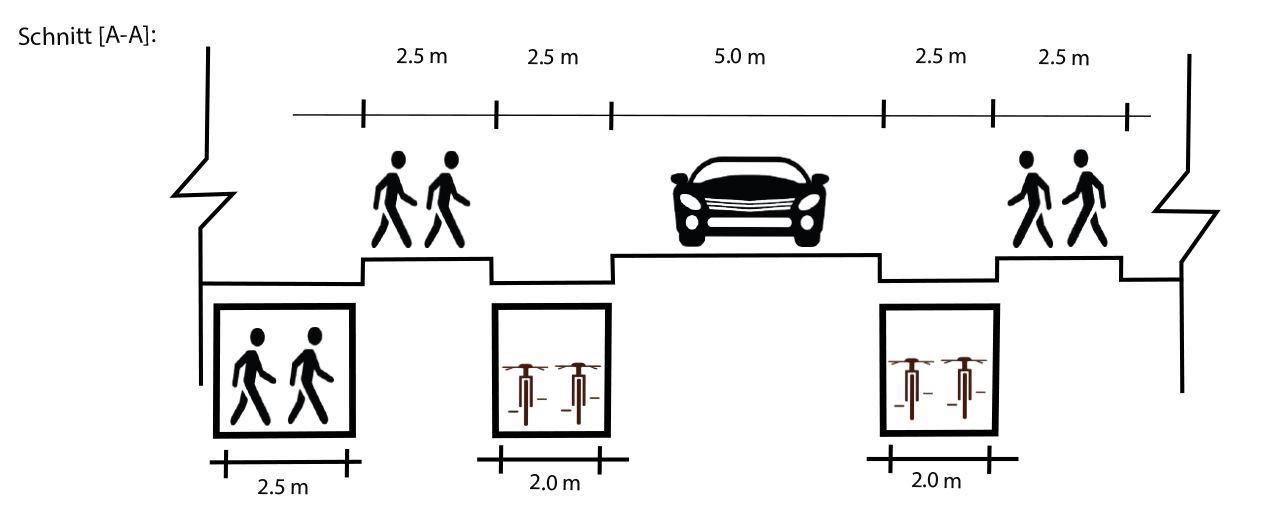
\includegraphics[width=0.7\textwidth]{figures/f-04-05-03-b-V3}
	\caption[Querschnitt Variante 3]{Querschnitt im Schnitt A-A der Variante 3}
	\label{img:V3Q}
\end{figure}

Die Baukosten der Variante 3 belaufen sich auf insgesamt 1.51 Mio CHF und werden wie für Variante 2 erläutert berechnet. Für den Bau der Unterführung unter dem Lastfall Eisenbahn und das Anbringen der Velostreifen sind 988'000 CHF vorgesehen und für den Bau der vier Rampen fallen 520'000 CHF an. (\cite{Baukosten2010}) 


In Tabelle \ref{tab:t-08-01-Varianten} werden die, für die Berechnung der Kosten verwendeten Eigenschaften der Varianten zusammengefasst.
%=============================================================================
% Thesis Template in LaTex
%
% File:  t-05-01-IsingModel.tex -- Table for the Ising
% Author(s): Juergen Hackl <hackl@ibi.baug.ethz.ch>
%            Clemens Kielhauser <kielhauser@ibi.baug.ethz.ch>
%
% Creation:  27 Jan 2014
% Time-stamp: <Tue 2013-08-13 20:14 juergen>
%
% Copyright (c) 2014 Infrastructure Management Group (IMG)
%               http://ibi.ethz.ch
%
% More information on LaTeX: http://www.latex-project.org/
%=============================================================================
%\small\renewcommand{\arraystretch}{1.2} 
%


\begin{table}[h!]
\scriptsize
{\setstretch{0.6}
%\renewcommand{\arraystretch}{1.4}
\flushleft
\begin{tabular}{@{}p{5cm} p{2.5cm} p{2.5cm} p{2.5cm}@{}} \\   
\toprule 		
\textbf{Eigenschaften}  				   								&\textbf{Variante\,1}  & \textbf{Variante\,2} & \textbf{Variante\,3}   \\			
\midrule 
Länge Fahrbahn ($m$)         	 		   								& 80                    & 80    			   & 80             	\\
Länge Unterführung ($m$)       	 		   								& -                     & 55    			   & 65             	\\
Velospuren:					   											&  2				    &  2				   &  4         		\\
Fahrbahnen									 		   					&  2				    &  2				   &  1         		\vspace*{0.25mm} \\
Breite eines Veloweg ($m$):				   								&  1.5				    &  1.5				   &  2         		\\
Breite einer Fahrbahn ($m$):			 		   					    &  3.5				    &  3				   &  5         		\vspace*{0.25mm} \\
Tempolimit	($\frac{km}{h}$) 		   						    		& 50				    & 30				   & 30                	\\
\underline{$\varnothing$\,Geschwindigkeit} ($\frac{km}{h}$) 			&       	            &   				   &               		 \\
\hspace*{5mm}\textbullet\, Velo            		       					& 15  					& 20    			   & 25      			\\
\hspace*{5mm}\textbullet\, MIV            		       					& 37  					& 30    			   & 30      			\vspace*{0.25mm} \\
\underline{Kapazität} ($\frac{Fahrzeug}{h}$)		        			&    				    &  				       &                  	 \\
\hspace*{5mm}\textbullet\, Velo            	       					    & 3350 					& 3767    			   & 4600      			\\
\hspace*{5mm}\textbullet\, MIV         		       					    & 2500 					& 2500    			   & 1250      			\\
\underline{Wartezeit} ($Minuten$)        		    			   		&    				    &  				       &                  	 \\
\hspace*{5mm}\textbullet\, Velo            	       					    & 5 					& 5    			       & 7      			\\
\hspace*{5mm}\textbullet\, MIV         		       					    & 5  					& 0      			   & 0      			\\
Baukosten ($CHF$)														& 68'000				& 1.16 Mio.			   & 1.51 Mio.           \\
\bottomrule

\end{tabular}
\caption{Basis Informationen der Varianten}
\label{tab:t-08-01-Varianten}
}
\end{table}


%=============================================================================
% EOF
%

%%% Local Variables:
%%% mode: latex
%%% TeX-master: "../guidelines"
%%% End:



\pagebreak

% ===========================================================================
% EOF
%

%%% Local Variables:
%%% mode: latex
%%% TeX-master: "../main"
%%% End:
